% Immutable derivative of the approved representative sample.
% PDF pages 37--50 / printed pages 23--36; bytes below are copied without translation changes.
\SampleSourcePage{37}{23}
\begin{Proof}
该证明基于 Banach 的闭值域定理. 首先注意到,
$-\Grad\in\cL(L^2(\Omega);H^{-1}(\Omega)^N)$ 是
$\Div\in\cL(H_0^1(\Omega)^N;L^2(\Omega))$ 的对偶算子. 又因为
$\Ran(\Grad)$ 是 $H^{-1}(\Omega)^N$ 的闭子空间, 所以可以应用 Banach 的闭值域定理(例如见 Yosida [84]):
\[
  \Ran(\Grad)=(\Ker(\Div))^0=V^0,
\]
其中 $V^0$ 表示 $V$ 的极集:
\begin{equation}\label{eq:sec2-polar-set}
  V^0=\{\mathbf y\in H^{-1}(\Omega)^N;\ \langle\mathbf y,\boldsymbol\phi\rangle=0
  \quad\forall\boldsymbol\phi\in V\}.
\end{equation}
这恰好就是所述引理的结论.
\end{Proof}

下一个推论给出 $V^\perp$ 的一个刻画. 在此之前需要先给出一个定义.

\setcounter{statement}{0}
\begin{Definition}\label{def:sec2-greens-operator}
令 $(-\Delta)^{-1}\in\cL(H^{-1}(\Omega)^N;H_0^1(\Omega)^N)$ 表示与
$\R^N$ 中 $-\Delta$ 的齐次 Dirichlet 问题对应的 Green 算子, 即
$\mathbf u=(-\Delta)^{-1}\mathbf f$ 当且仅当 $\mathbf u$ 是下列问题的解:
\[
  -\Delta\mathbf u=\mathbf f\quad\text{in }\Omega,
  \qquad \mathbf u=0\quad\text{on }\Gamma.
\]
\end{Definition}

\setcounter{statement}{2}
\begin{Corollary}\label{cor:sec2-vperp-green}
有
\[
  V^\perp=\{(-\Delta)^{-1}\Grad q;\ q\in L^2(\Omega)\}.
\]
\end{Corollary}
\begin{Proof}
首先, 容易验证对每个 $q\in L^2(\Omega)$ 都有
$(-\Delta)^{-1}\Grad q\in V^\perp$. 反之, 令 $\mathbf u\in V^\perp$, 并在
$H_0^1(\Omega)^N$ 上定义线性泛函 $l$:
$\langle l,\mathbf v\rangle=(\Grad\mathbf u,\Grad\mathbf v)$. 它属于
$H^{-1}(\Omega)^N$ 且在 $V$ 上为零. 因此, 由
Lemma~\ref{lem:sec2-hminus1-gradient-coarse}, 存在
$p\in L^2(\Omega)$ 使得
\[
  \langle l,\mathbf v\rangle=(\Grad\mathbf u,\Grad\mathbf v)
  =\langle\Grad p,\mathbf v\rangle
  \quad\forall\mathbf v\in H_0^1(\Omega)^N.
\]
故 $\mathbf u$ 确实具有表示 $\mathbf u=(-\Delta)^{-1}\Grad p$.
\end{Proof}

现在注意到, Green 公式 \eqref{eq:green-first-identity-component} 给出
\[
  \int_\Omega \Div\mathbf v\dd x=0
  \quad\forall\mathbf v\in H_0^1(\Omega)^N.
\]
因此 $\Div$ 的值域包含于 $L^2(\Omega)$ 的一个真闭子空间中. 为方便起见, 记该子空间为
\[
  L_0^2(\Omega)=\left\{p\in L^2(\Omega);\ \int_\Omega p\dd x=0\right\}.
\]
$L_0^2(\Omega)$ 的用处特别体现在
\begin{equation}\label{eq:sec2-l20-quotient-norm}
  \|q\|_{0,\Omega}=\inf_{c\in\R}\|q+c\|_{0,\Omega}
  =\|\dot q\|_{L^2(\Omega)/\R}
  \quad\forall q\in L_0^2(\Omega).
\end{equation}

\SampleSourcePage{38}{24}
于是 $L_0^2(\Omega)$ 可以与 $L^2(\Omega)/\R$ 等距同一. 下一个推论进一步说明,
$\Div$ 的值域恰好是 $L_0^2(\Omega)$.

\setcounter{statement}{3}
\begin{Corollary}\label{cor:sec2-grad-div-isomorphisms}
设 $\Omega$ 连通. 则:

1) 算子 $\Grad$ 是从 $L_0^2(\Omega)$ 到 $V^0$ 的同构;

2) 算子 $\Div$ 是从 $V^\perp$ 到 $L_0^2(\Omega)$ 的同构.
\end{Corollary}
\begin{Proof}
1) 已知 $\Grad\in\cL(L_0^2(\Omega);V^0)$, 而
Lemma~\ref{lem:sec2-hminus1-gradient-coarse} 断言该映射是双射.
由于 $V^0$ 和 $L_0^2(\Omega)$ 都是 Banach 空间, $\Grad$ 是同构.

2) 由 1), 并利用 $\Div$ 是 $-\Grad$ 的对偶算子, 可知 $\Div$ 是从
$(V^0)'$ 到 $(L_0^2(\Omega))'$ 的同构. 现在只需证明 $V^0$ 可与
$(V^\perp)'$ 同一. 任取 $g\in(V^\perp)'$, 令
\[
  \langle\widetilde g,\mathbf v\rangle=\langle g,\mathbf v^\perp\rangle
  \quad\forall\mathbf v\in H_0^1(\Omega)^N,
\]
其中 $\mathbf v^\perp$ 是 $\mathbf v$ 在 $V^\perp$ 上的正交投影. 显然
$\widetilde g\in V^0$, 且线性映射 $g\mapsto\widetilde g$ 将
$(V^\perp)'$ 等距映到 $V^0$ 上. 因而可以同一 $(V^\perp)'$ 与 $V^0$.
\end{Proof}

\setcounter{statement}{0}
\begin{Remark}\label{rem:sec2-abstract-div-isomorphism}
Corollary~\ref{cor:sec2-grad-div-isomorphisms} 的 2) 的证明在抽象情形中仍然有效
(见 Lemma~\ref{lem:ch4-abstract-div}).
\end{Remark}

仍用 $\mathbf n$ 表示 $\Gamma$ 的外单位法向量. 下一个引理利用无散函数给出边界值的提升算子.

\setcounter{statement}{1}
\begin{Lemma}\label{lem:sec2-div-free-lifting}
设 $\Omega$ 连通. 对每个满足 $\int_\Gamma\mathbf g\cdot\mathbf n\dd s=0$ 的
$\mathbf g\in H^{1/2}(\Gamma)^N$, 存在 $\mathbf u\in H^1(\Omega)^N$, 在加上
$V$ 中函数的意义下唯一, 使得
\[
  \Div\mathbf u=0\quad\text{in }\Omega,
  \qquad \mathbf u=\mathbf g\quad\text{on }\Gamma.
\]
此外,
\begin{equation}\label{eq:sec2-div-free-lifting-bound}
  \inf_{\mathbf v\in V}\|\mathbf u+\mathbf v\|_{1,\Omega}
  \le C\|\mathbf g\|_{1/2,\Gamma},
\end{equation}
其中常数 $C>0$ 与 $\mathbf u$ 和 $\mathbf g$ 无关.
\end{Lemma}
\begin{Proof}
显然, 这种函数 $\mathbf u$ 在 $[H^1(\Omega)^N]/V$ 中必须唯一. 下面验证其存在性.
任取满足 $\mathbf w=\mathbf g$ on $\Gamma$ 的 $\mathbf w\in H^1(\Omega)^N$.
Green 公式 \eqref{eq:green-first-identity-component} 给出
\[
  \int_\Omega\Div\mathbf w\dd x
  =\int_\Gamma\mathbf g\cdot\mathbf n\dd s=0.
\]
因此 $\Div\mathbf w\in L_0^2(\Omega)$. 由 Corollary~\ref{cor:sec2-grad-div-isomorphisms} 的 2),
存在唯一的 $\mathbf v\in V^\perp$ 使得
\[
  \Div\mathbf v=\Div\mathbf w.
\]

\SampleSourcePage{39}{25}
并且
\[
  \|\mathbf v\|_{1,\Omega}\le C_1\|\Div\mathbf w\|_{0,\Omega}.
\]
显然,
\[
  \mathbf u=\mathbf w-\mathbf v
\]
就是所需函数. 还需验证估计 \eqref{eq:sec2-div-free-lifting-bound}. 首先注意到
\[
  \|\mathbf u\|_{1,\Omega}\le C_2\|\mathbf w\|_{1,\Omega},
\]
其中 $C_2>0$ 与 $\mathbf u$ 和 $\mathbf w$ 无关. 对此不等式两边取下确界, 并使用
$H^{1/2}(\Gamma)$ 上的范数 \eqref{eq:trace-space-norm}, 即得
\eqref{eq:sec2-div-free-lifting-bound}.
\end{Proof}

下述定理加强了 Lemma~\ref{lem:sec2-hminus1-gradient-coarse} 的结论,
是 Stokes 方程理论中的基本工具. 它是 De Rham 定理
Theorem~\eqref{eq:de-rham-distributional-principle} 的一个简化版本, 但对我们的目的已经足够.

\setcounter{statement}{2}
\begin{Theorem}\label{thm:sec2-gradient-characterization}
若 $\mathbf f\in H^{-1}(\Omega)^N$ 满足
\begin{equation}\label{eq:sec2-annihilates-test-divfree}
  \langle\mathbf f,\boldsymbol\phi\rangle=0
  \quad\forall\boldsymbol\phi\in\mathcal V,
\end{equation}
则存在 $p\in L^2(\Omega)$ 使得
\[
  \mathbf f=\Grad p.
\]
若 $\Omega$ 连通, 则 $p$ 在相差一个加性常数的意义下唯一.
\end{Theorem}
\begin{Proof}
暂设 $\Omega$ 连通. 先证明对某个 $p\in L_{\loc}^2(\Omega)$ 有
$\mathbf f=\Grad p$; 随后 Corollary~\ref{cor:local-l2-gradient-global-l2}
立即给出 $p\in L^2(\Omega)$.

由于 $\Omega$ 是有界、连通且 Lipschitz 连续的开集, 存在由连通 Lipschitz 连续开集组成的递增序列
$(\Omega_m)_{m\ge1}$, 使得
\[
  \overline{\Omega_m}\subset\Omega,
  \qquad \Omega=\bigcup_{m\ge1}\Omega_m.
\]
取 $\mathbf u_m\in H_0^1(\Omega)^N$, 满足
\[
  \mathbf u_m=0\quad\text{outside }\Omega_m,
  \qquad \Div\mathbf u_m=0.
\]
为了应用 Lemma~\ref{lem:sec2-hminus1-gradient-coarse}, 需要将
$\mathbf u_m$ 正则化且保持无散. 这由经典的磨光子方法实现(例如见 Adams [1]):
对 $\varepsilon>0$, 令 $\rho_\varepsilon$ 是 $\D(\R^N)$ 中的正则化序列,
当 $\|x\|>\varepsilon$ 时为零, 且满足
\[
  \rho_\varepsilon(x)\ge0,
  \qquad\int_{\R^N}\rho_\varepsilon(x)\dd x=1,
  \qquad\lim_{\varepsilon\to0}\rho_\varepsilon=\delta
  \quad\text{in }\D'(\R^N).
\]

\SampleSourcePage{40}{26}
卷积的性质给出
\[
\begin{gathered}
  \Div(\rho_\varepsilon*\mathbf u_m)
  =\rho_\varepsilon*\Div\mathbf u_m=0,\\
  \rho_\varepsilon*\mathbf u_m\in\D(\Omega)^N
  \quad\text{if }\varepsilon\text{ is sufficiently small},\\
  \lim_{\varepsilon\to0}(\rho_\varepsilon*\mathbf u_m)
  =\mathbf u_m\quad\text{in }H^1(\Omega)^N.
\end{gathered}
\]
所以由 \eqref{eq:sec2-annihilates-test-divfree},
\[
  \langle\mathbf f,\mathbf u_m\rangle
  =\lim_{\varepsilon\to0}\langle\mathbf f,\rho_\varepsilon*\mathbf u_m\rangle=0.
\]
因此, Lemma~\ref{lem:sec2-hminus1-gradient-coarse} 蕴含存在
$p_m\in L^2(\Omega_m)$ 使得
\[
  \mathbf f=\Grad p_m\quad\text{in }\Omega_m.
\]
因为在 $\Omega_m$ 上 $\Grad p_m=\Grad p_{m+1}$, 所以 $p_m-p_{m+1}$ 在
$\Omega_m$ 上为常数. 又因 $p_m$ 只在相差一个加性常数的意义下唯一, 可选择该常数使
\[
  p_{m+1}=p_m\quad\text{in }\Omega_m\quad\forall m\ge1.
\]
于是存在 $p\in L_{\loc}^2(\Omega)$ 使得
\[
  \mathbf f=\Grad p\quad\text{in }\Omega.
\]
当 $\Omega$ 不连通时, 对它的每个连通分支分别应用上述论证.
\end{Proof}

\setcounter{statement}{4}
\begin{Corollary}\label{cor:sec2-test-divfree-dense}
空间 $\mathcal V$ 在 $V$ 中关于 $H_0^1(\Omega)^N$ 的范数稠密.
\end{Corollary}
\begin{Proof}
证明基于 Banach 空间的如下性质:
\begin{equation}\label{eq:sec2-banach-density-criterion}
\left\{
\begin{minipage}{0.72\linewidth}
Banach 空间 $M$ 的子空间 $\mathcal M$ 在 $M$ 中稠密, 当且仅当
$M'$ 中每个在 $\mathcal M$ 上为零的元素也在 $M$ 上为零.
\end{minipage}
\right.
\end{equation}
首先, 注意到 $H^{-1}(\Omega)^N$ 中每个在 $\mathcal V$ 上为零的
$\mathbf f$ 也在 $V$ 上为零. 事实上, 由 Theorem~\ref{thm:sec2-gradient-characterization},
$\mathbf f$ 必为 $\mathbf f=\Grad p$ 的形式, 其中 $p\in L^2(\Omega)$.
又因为 $V$ 在 $H_0^1(\Omega)^N$ 中闭, $V'$ 可与 $H^{-1}(\Omega)^N$ 的一个子空间同一,
结论由 \eqref{eq:sec2-banach-density-criterion} 得出.
\end{Proof}

到目前为止, 我们主要关心 $H^1(\Omega)^N$ 的子空间; 但以后使用正则性较低的函数会很有价值.
为此引入
\[
  H(\Div;\Omega)=\{\mathbf v\in L^2(\Omega)^N;\ \Div\mathbf v\in L^2(\Omega)\},
\]
它关于范数
\begin{equation}\label{eq:sec2-hdiv-norm}
  \|\mathbf v\|_{H(\Div;\Omega)}
  =\{\|\mathbf v\|_{0,\Omega}^2+\|\Div\mathbf v\|_{0,\Omega}^2\}^{1/2}
\end{equation}
显然是 Hilbert 空间; 并令
\[
  H_0(\Div;\Omega)=\overline{\D(\Omega)^N}^{\,H(\Div;\Omega)}.
\]

\SampleSourcePage{41}{27}
\setcounter{statement}{3}
\begin{Theorem}\label{thm:sec2-dense-in-hdiv}
设 $\Omega$ 是 $\R^N$ 的 Lipschitz 连续开子集(不必有界). 则
$\D(\overline\Omega)^N$ 在 $H(\Div;\Omega)$ 中稠密.
\end{Theorem}
\begin{Proof}
证明仍基于性质 \eqref{eq:sec2-banach-density-criterion}. 设
$l\in(H(\Div;\Omega))'$. 因为 $H(\Div;\Omega)$ 是 Hilbert 空间, 可将 $l$
与某个 $\mathbf l\in H(\Div;\Omega)$ 对应, 使得
\[
  \langle l,\mathbf u\rangle
  =\sum_{i=1}^{N}(l_i,u_i)+(l_{N+1},\Div\mathbf u)
  \quad\forall\mathbf u\in H(\Div;\Omega),
\]
其中 $l_{N+1}=\Div\mathbf l$. 假定 $l$ 在 $\D(\overline\Omega)^N$ 上为零,
并以 $\widetilde l_i$ 表示 $l_i$ 在 $\Omega$ 外的零延拓. 上式可改写为
\[
  \int_{\R^N}\left\{\sum_{i=1}^{N}\widetilde l_i\phi_i
  +\widetilde l_{N+1}\Div\boldsymbol\phi\right\}\dd x=0
  \quad\forall\boldsymbol\phi\in\D(\R^N)^N.
\]
这意味着在 $\R^N$ 上的分布意义下
\[
  \widetilde{\mathbf l}=\Grad\widetilde l_{N+1}.
\]
由于 $\widetilde{\mathbf l}\in L^2(\R^N)^N$, 有
$\widetilde l_{N+1}\in H^1(\R^N)$. 由
Theorem~\ref{thm:sobolev-density-extension} $2^\circ)$, 可知
$l_{N+1}\in H_0^1(\Omega)$. 因 $\D(\Omega)$ 在 $H_0^1(\Omega)$ 中稠密,
取 $\psi_\mu\in\D(\Omega)$ 使 $\psi_\mu\to l_{N+1}$ in $H^1(\Omega)$. 则
\[
  \langle l,\mathbf u\rangle
  =\lim_{\mu\to\infty}\{(\Grad\psi_\mu,\mathbf u)
  +(\psi_\mu,\Div\mathbf u)\}=0
  \quad\forall\mathbf u\in H(\Div;\Omega).
\]
故若 $l$ 在 $\D(\overline\Omega)^N$ 上为零, 它也在 $H(\Div;\Omega)$ 上为零,
从而得到所需稠密性.
\end{Proof}

下面的定理涉及 $H(\Div;\Omega)$ 中函数边界值的法向分量.

\setcounter{statement}{4}
\begin{Theorem}\label{thm:sec2-normal-trace}
定义在 $\D(\overline\Omega)^N$ 上的映射
$\gamma_n:\mathbf v\mapsto\mathbf v\cdot\mathbf n|_\Gamma$ 可以连续延拓为从
$H(\Div;\Omega)$ 到 $H^{-1/2}(\Gamma)$ 的线性连续映射, 延拓后仍记为 $\gamma_n$.
\end{Theorem}
\begin{Proof}
令 $\phi\in\D(\overline\Omega)$ 且 $\mathbf v\in\D(\overline\Omega)^N$. 有 Green 公式
\[
  (\mathbf v,\Grad\phi)+(\Div\mathbf v,\phi)
  =\int_\Gamma\phi\,\mathbf v\cdot\mathbf n\dd s.
\]
由于 $\D(\overline\Omega)$ 在 $H^1(\Omega)$ 中稠密, 对
$\phi\in H^1(\Omega)$ 和 $\mathbf v\in\D(\overline\Omega)^N$ 上式仍成立. 因而
\[
  \left|\int_\Gamma\phi\,\mathbf v\cdot\mathbf n\dd s\right|
  \le\|\mathbf v\|_{H(\Div;\Omega)}\|\phi\|_{1,\Omega}.
\]

\SampleSourcePage{42}{28}
任取 $\mu\in H^{1/2}(\Gamma)$. 存在 $\phi\in H^1(\Omega)$ 满足
$\phi=\mu$ on $\Gamma$. 因而
\[
  \left|\int_\Gamma\mu\,\mathbf v\cdot\mathbf n\dd s\right|
  \le\|\mathbf v\|_{H(\Div;\Omega)}\|\mu\|_{1/2,\Gamma},
\]
于是
\[
  \|\mathbf v\cdot\mathbf n\|_{-1/2,\Gamma}
  \le\|\mathbf v\|_{H(\Div;\Omega)}.
\]
所以 $\gamma_n$ 关于 $H(\Div;\Omega)$ 的范数连续. 由
Theorem~\ref{thm:sec2-dense-in-hdiv}, 它可连续延拓为映射
\[
  \gamma_n\in\cL(H(\Div;\Omega);H^{-1/2}(\Gamma)),
\]
且
\begin{equation}\label{eq:sec2-normal-trace-norm}
  \|\gamma_n\|_{\cL(H(\Div;\Omega);H^{-1/2}(\Gamma))}\le1.
\end{equation}
\end{Proof}

延拓后, $\gamma_n\mathbf v$ 称为 $\mathbf v$ 在 $\Gamma$ 上的法向分量, 简记为
$\mathbf v\cdot\mathbf n$. 由 Theorem~\ref{thm:sec2-dense-in-hdiv} 和
Theorem~\ref{thm:sec2-normal-trace} 得到 Green 公式
\begin{equation}\label{eq:sec2-hdiv-green}
  (\mathbf v,\Grad\phi)+(\Div\mathbf v,\phi)
  =\langle\mathbf v\cdot\mathbf n,\phi\rangle_\Gamma
  \quad\forall\mathbf v\in H(\Div;\Omega),\ \forall\phi\in H^1(\Omega).
\end{equation}
因此可将 Laplace 算子的 Green 公式推广到更广的函数范围.

\setcounter{statement}{5}
\begin{Corollary}\label{cor:sec2-laplace-green}
设 $u\in H^1(\Omega)$ 且 $\Delta u\in L^2(\Omega)$. 则
$\partial u/\partial n\in H^{-1/2}(\Gamma)$, 并且
\begin{equation}\label{eq:sec2-laplace-green}
  (\Grad u,\Grad v)=-(\Delta u,v)
  +\langle\partial u/\partial n,v\rangle_\Gamma
  \quad\forall v\in H^1(\Omega).
\end{equation}
\end{Corollary}
证明留作练习.

另一个有趣的结果是, 现在可以恰当地解释
Section~\ref{subsec:laplace-neumann-example} 的变分问题 $(N')$,
并证明它与 Neumann 问题 $(N)$ 等价. 证明由 \eqref{eq:sec2-laplace-green} 立即得到, 故略去.

\setcounter{statement}{6}
\begin{Corollary}\label{cor:sec2-neumann-equivalence}
问题 \eqref{eq:neumann-variational-problem} 与问题
\eqref{eq:laplace-neumann-pde},
\eqref{eq:laplace-neumann-boundary},
\eqref{eq:laplace-neumann-compatibility} 等价.
\end{Corollary}

下面两个结果给出关于 $\gamma_n$ 的进一步信息.

\setcounter{statement}{7}
\begin{Corollary}\label{cor:sec2-normal-trace-surjective}
有
\[
  \Ran(\gamma_n)=H^{-1/2}(\Gamma),
\]
并且
\[
  \|\gamma_n\|_{\cL(H(\Div;\Omega);H^{-1/2}(\Gamma))}=1.
\]
\end{Corollary}
\begin{Proof}
令 $\mu\in H^{-1/2}(\Gamma)$. 需要构造 $\mathbf v\in H(\Div;\Omega)$, 使
\[
  \mathbf v\cdot\mathbf n=\mu\quad\text{on }\Gamma,
  \qquad \|\mathbf v\cdot\mathbf n\|_{-1/2,\Gamma}
  \ge\|\mathbf v\|_{H(\Div;\Omega)}.
\]

\SampleSourcePage{43}{29}
结合 \eqref{eq:sec2-normal-trace-norm}, 这将证明该推论. 考虑问题: 求
$\phi\in H^1(\Omega)$ 使
\[
  -\Delta\phi+\phi=0\quad\text{in }\Omega,
  \qquad \partial\phi/\partial n=\mu\quad\text{on }\Gamma.
\]
与 Section~\ref{subsec:laplace-neumann-example} 的 Neumann 问题不同,
该问题在 $H^1(\Omega)$ 中恰有一个解 $\phi$. 令 $\mathbf v=\Grad\phi$. 则
$\mathbf v\in H(\Div;\Omega)$ 且 $\mathbf v\cdot\mathbf n=\mu$. 此外
\[
  |\phi|_{1,\Omega}^2=\langle\mu,\phi\rangle_\Gamma
  \le\|\mu\|_{-1/2,\Gamma}\|\phi\|_{1,\Omega}.
\]
由于 $\Div\mathbf v=\phi$, 有
\[
  \|\mathbf v\|_{H(\Div;\Omega)}
  \le\|\mu\|_{-1/2,\Gamma}
  =\|\mathbf v\cdot\mathbf n\|_{-1/2,\Gamma}.
\]
\end{Proof}

\setcounter{statement}{5}
\begin{Theorem}\label{thm:sec2-h0div-kernel}
有
\[
  H_0(\Div;\Omega)=\Ker(\gamma_n)
  =\{\mathbf u\in H(\Div;\Omega);\ \mathbf u\cdot\mathbf n|_\Gamma=0\}.
\]
\end{Theorem}
\begin{Proof}
先证明 $\D(\Omega)^N$ 在 $\Ker(\gamma_n)$ 中稠密. 再次使用性质
\eqref{eq:sec2-banach-density-criterion}. 令 $l\in(\Ker(\gamma_n))'$, 并令
$\mathbf l\in\Ker(\gamma_n)$ 由下式与 $l$ 对应:
\begin{equation}\label{eq:sec2-kernel-functional}
  \langle l,\mathbf u\rangle
  =\sum_{i=1}^{N}(l_i,u_i)+(l_{N+1},\Div\mathbf u)
  \quad\forall\mathbf u\in\Ker(\gamma_n).
\end{equation}
假设 $l$ 在 $\D(\Omega)^N$ 上为零. 这意味着
\[
  \mathbf l=\Grad l_{N+1}.
\]
故 $l_{N+1}\in H^1(\Omega)$, 可将 Green 公式 \eqref{eq:sec2-hdiv-green}
应用于 \eqref{eq:sec2-kernel-functional}:
\[
  \langle l,\mathbf u\rangle
  =\langle\mathbf u\cdot\mathbf n,l_{N+1}\rangle_\Gamma
  \quad\forall\mathbf u\in\Ker(\gamma_n).
\]
因此 $l$ 在 $\Ker(\gamma_n)$ 上也为零, 从而
$\Ker(\gamma_n)\subset H_0(\Div;\Omega)$. 反向包含由 Green 公式
\eqref{eq:sec2-hdiv-green} 立即得到.
\end{Proof}

最后考察 $H_0(\Div;\Omega)$ 中无散函数的子空间
\[
  H=\{\mathbf u\in H_0(\Div;\Omega);\ \Div\mathbf u=0\}.
\]
因为它是 $L^2(\Omega)^N$ 的闭子空间, 有分解
\[
  L^2(\Omega)^N=H\oplus H^\perp,
\]
其中 $H^\perp$ 表示 $H$ 关于内积 $(\cdot,\cdot)$ 在 $L^2(\Omega)^N$ 中的正交补.
下一个定理刻画 $H^\perp$.

\SampleSourcePage{44}{30}
\setcounter{statement}{6}
\begin{Theorem}\label{thm:sec2-hperp-gradients}
若 $\Omega$ 连通, 则
\[
  H^\perp=\{\Grad q;\ q\in H^1(\Omega)\}.
\]
\end{Theorem}
\begin{Proof}
为简便起见, 记 $X=\{\Grad q;q\in H^1(\Omega)\}$. 由
Theorem~\ref{thm:h1-quotient-hilbert},
$X$ 是 $L^2(\Omega)^N$ 的闭子空间. 因此若证明 $X^\perp=H$, 则
\[
  H^\perp=(X^\perp)^\perp=\overline X=X,
\]
即得结论.

先令 $\mathbf u\in H$. 公式 \eqref{eq:sec2-hdiv-green} 和
Theorem~\ref{thm:sec2-h0div-kernel} 给出
\[
  (\mathbf u,\Grad q)=0\quad\forall q\in H^1(\Omega).
\]
故 $H\subset X^\perp$. 反之, 若 $\mathbf u\in L^2(\Omega)^N$ 且
\[
  (\mathbf u,\Grad q)=0\quad\forall q\in H^1(\Omega),
\]
取 $q\in\D(\Omega)$ 即得 $\Div\mathbf u=0$, 因此
$\mathbf u\in H(\Div;\Omega)$. 再由 \eqref{eq:sec2-hdiv-green} 得
$\mathbf u\cdot\mathbf n=0$. 由 Theorem~\ref{thm:sec2-h0div-kernel},
$\mathbf u\in H$, 故 $X^\perp\subset H$.
\end{Proof}

\setcounter{statement}{7}
\begin{Theorem}\label{thm:sec2-test-space-dense-h}
空间 $\mathcal V$ 在 $H$ 中稠密.
\end{Theorem}
\begin{Proof}
这仍是性质 \eqref{eq:sec2-banach-density-criterion} 的应用. 令
$l\in H'$ 并令 $\mathbf l\in H$ 满足
\[
  \langle l,\mathbf u\rangle=(\mathbf l,\mathbf u)
  \quad\forall\mathbf u\in H.
\]
若 $l$ 在 $\mathcal V$ 上为零, 则 $\mathbf l$ 满足
Theorem~\ref{thm:sec2-gradient-characterization} 的假设, 因而
\[
  \mathbf l=\Grad p
\]
对某个 $p\in L^2(\Omega)$ 成立. 因 $\mathbf l\in L^2(\Omega)^N$, 有
$p\in H^1(\Omega)$. 于是 \eqref{eq:sec2-hdiv-green} 给出
\[
  \langle l,\mathbf u\rangle
  =-(p,\Div\mathbf u)+\langle\mathbf u\cdot\mathbf n,p\rangle_\Gamma=0
  \quad\forall\mathbf u\in H.
\]
\end{Proof}

\setcounter{subsection}{2}
\subsection{与 curl 算子有关的空间的若干性质}\label{subsec:sec2-curl-spaces}
除非另有说明, 本小节假定维数 $N$ 为 2 或 3, 且 $\Omega$ 是 $\R^N$ 中具有
Lipschitz 连续边界 $\Gamma$ 的有界区域. 当 $N=2$ 时, 对
$\phi\in\D'(\Omega)$ 和 $\mathbf v\in\D'(\Omega)^2$ 定义
\[
  \Curl\phi=\left(\frac{\partial\phi}{\partial x_2},
  -\frac{\partial\phi}{\partial x_1}\right),
  \qquad
  \Curl\mathbf v=\frac{\partial v_2}{\partial x_1}
  -\frac{\partial v_1}{\partial x_2}.
\]

\SampleSourcePage{45}{31}
当 $N=3$ 时, 对 $\mathbf v\in\D'(\Omega)^3$ 定义
\[
  \Curl\mathbf v=\left(
  \frac{\partial v_3}{\partial x_2}-\frac{\partial v_2}{\partial x_3},
  \frac{\partial v_1}{\partial x_3}-\frac{\partial v_3}{\partial x_1},
  \frac{\partial v_2}{\partial x_1}-\frac{\partial v_1}{\partial x_2}
  \right).
\]
容易验证恒等式
\[
  \Curl(\Curl\phi)=-\Delta\phi\quad(N=2),
\]
以及
\[
  \left.\begin{array}{ll}
  \Curl(\Curl\mathbf v)=-\Delta\mathbf v+\Grad(\Div\mathbf v),&N=3,\\
  \Curl(\Curl\mathbf v)=-\Delta\mathbf v+\Grad(\Div\mathbf v),&N=2.
  \end{array}\right\}
\]
注意二维向量场的 curl 是标量. 为避免引入过多记号, 在不会混淆时仍约定把它记成向量形式.

首先推广经典 Stokes 定理: 若一个 $\mathcal C^1$ 函数在 $\R^N$ 的单连通区域中 curl 为零,
则该函数是一个梯度.

\setcounter{statement}{8}
\begin{Theorem}\label{thm:sec2-curl-free-gradient}
再假设 $\Omega$ 单连通. 函数 $\mathbf u\in L^2(\Omega)^N$ 满足
$\Curl\mathbf u=0$ in $\Omega$, 当且仅当存在唯一的
$p\in H^1(\Omega)/\R$ 使得
\[
  \mathbf u=\Grad p.
\]
\end{Theorem}
\begin{Proof}
证明与 Theorem~\ref{thm:sec2-gradient-characterization} 非常相似: 先证明对某个
$p\in L_{\loc}^2(\Omega)$ 有 $\mathbf u=\Grad p$, 再应用
Corollary~\ref{cor:local-l2-gradient-global-l2} 得到
$p\in L^2(\Omega)$. 显然 $p\in H^1(\Omega)$, 且在 $H^1(\Omega)/\R$ 中唯一.

仍可取由单连通 Lipschitz 连续开集组成的递增序列 $(\Omega_m)_{m\ge1}$, 满足
\[
  \overline{\Omega_m}\subset\Omega,
  \qquad\Omega=\bigcup_{m\ge1}\Omega_m.
\]
思路是将 $\mathbf u$ 正则化, 使其在 $\Omega_m$ 上的限制仍有零 curl, 然后对这个光滑函数应用 Stokes 定理.
对 $\varepsilon>0$, 令 $\rho_\varepsilon\in\D(\R^N)$ 是
Theorem~\ref{thm:sec2-gradient-characterization} 中引入的磨光子, 并令
$\widetilde{\mathbf u}$ 是 $\mathbf u$ 在 $\Omega$ 外的零延拓. 则

\SampleSourcePage{46}{32}
\begin{equation}\label{eq:sec2-curl-mollifier-properties}
\left\{\begin{aligned}
  &\rho_\varepsilon*\widetilde{\mathbf u}\in\D(\R^N)^N,\\
  &\lim_{\varepsilon\to0}(\rho_\varepsilon*\widetilde{\mathbf u})
    =\widetilde{\mathbf u}\quad\text{in }L^2(\R^N)^N,\\
  &\Curl(\rho_\varepsilon*\widetilde{\mathbf u})
    =\rho_\varepsilon*\Curl\widetilde{\mathbf u}.
\end{aligned}\right.
\end{equation}
若 $\varepsilon$ 足够小, 则
\[
  \bigcup_{x\in\Omega_m}B(x;\varepsilon)\subset\Omega,
\]
其中 $B(x;\varepsilon)$ 是以 $x$ 为中心、$\varepsilon$ 为半径的球. 因而
\[
  \Curl(\rho_\varepsilon*\widetilde{\mathbf u})=0
  \quad\text{in }\Omega_m.
\]
由 Stokes 定理, 存在光滑函数 $p_\varepsilon$(至少属于 $H^1(\Omega_m)$) 使
\[
  \rho_\varepsilon*\widetilde{\mathbf u}=\Grad p_\varepsilon
  \quad\text{in }\Omega_m.
\]
又由 \eqref{eq:sec2-curl-mollifier-properties}, 存在 $p_m\in H^1(\Omega_m)$ 使
\[
  \lim_{\varepsilon\to0}p_\varepsilon=p_m
  \quad\text{in }H^1(\Omega_m)/\R,
\]
且 $\mathbf u=\Grad p_m$ in $\Omega_m$. 余下证明与
Theorem~\ref{thm:sec2-gradient-characterization} 相同.
\end{Proof}

结合 Theorem~\ref{thm:sec2-hperp-gradients}, 得到 $H^\perp$ 的另一种刻画.

\setcounter{statement}{8}
\begin{Corollary}\label{cor:sec2-hperp-kernel-curl}
若 $\Omega$ 满足 Theorem~\ref{thm:sec2-curl-free-gradient} 的条件, 则在
$L^2(\Omega)^N$ 中
\[
  H^\perp=\Ker(\Curl)
  =\{\mathbf v\in L^2(\Omega)^N;\ \Curl\mathbf v=0\}.
\]
\end{Corollary}

\setcounter{statement}{1}
\begin{Remark}\label{rem:sec2-h-curlzero}
由 Corollary~\ref{cor:sec2-hperp-kernel-curl}, 若 $\mathbf u\in H$ 且
$\Curl\mathbf u=0$, 则 $\mathbf u=0$; 当然这里要求 $\Omega$ 有界且单连通.
\end{Remark}

如同定义 $H(\Div;\Omega)$ 一样, 定义
\[
  H(\Curl;\Omega)=\{\mathbf v\in L^2(\Omega)^N;
  \ \Curl\mathbf v\in L^2(\Omega)^N\},
\]
它关于范数
\[
  \|\mathbf v\|_{H(\Curl;\Omega)}
  =\{\|\mathbf v\|_{0,\Omega}^2+\|\Curl\mathbf v\|_{0,\Omega}^2\}^{1/2}
\]
是 Hilbert 空间, 并令
\[
  H_0(\Curl;\Omega)=\overline{\D(\Omega)^N}^{\,H(\Curl;\Omega)}.
\]
我们将为这些空间建立 Theorems~\ref{thm:sec2-dense-in-hdiv},
\ref{thm:sec2-normal-trace} 和 \ref{thm:sec2-h0div-kernel} 的对应结果, 先给出两个预备引理.

\SampleSourcePage{47}{33}
\setcounter{statement}{2}
\begin{Lemma}\label{lem:sec2-compact-support-dense-hcurl}
设 $\Omega$ 是 $\R^N$ 的 Lipschitz 连续开子集(不必有界). 则
$H(\Curl;\Omega)$ 中具有紧支集的函数集在 $H(\Curl;\Omega)$ 中稠密.
\end{Lemma}
\begin{Proof}
采用经典截断过程. 令 $\mathbf u\in H(\Curl;\Omega)$, 并取
$\phi\in\mathcal C^\infty(\R^N)$, 使 $0\le\phi\le1$ 且
\[
  \phi(x)=\begin{cases}
  1,&\|x\|\le1,\\
  0,&\|x\|\ge2.
  \end{cases}
\]
对任意实数 $a>0$, 作变量替换
\[
  \phi_a(x)=\phi(x/a).
\]
由于 $\phi_a$ 光滑, $\phi_a\mathbf u\in H(\Curl;\Omega)$; 此外
\[
  \lim_{a\to\infty}\phi_a\mathbf u=\mathbf u
  \quad\text{in }H(\Curl;\Omega),
\]
且 $\phi_a\mathbf u$ 的支集紧. 因而 $\phi_a\mathbf u$ 即为所需序列.
\end{Proof}

\setcounter{statement}{3}
\begin{Lemma}\label{lem:sec2-h0curl-characterization-test}
若 $\mathbf f\in H(\Curl;\Omega)$ 满足
\begin{equation}\label{eq:sec2-h0curl-test-identity}
  (\mathbf f,\Curl\boldsymbol\phi)-(\Curl\mathbf f,\boldsymbol\phi)=0
  \quad\forall\boldsymbol\phi\in\D(\overline\Omega)^N,
\end{equation}
则 $\mathbf f\in H_0(\Curl;\Omega)$.
\end{Lemma}
\begin{Proof}
令 $\widetilde{\mathbf f}$ 表示 $\mathbf f$ 在 $\Omega$ 外的零延拓. 首先,
\eqref{eq:sec2-h0curl-test-identity} 蕴含
$\widetilde{\mathbf f}\in H(\Curl;\R^N)$. 为构造在
$H(\Curl;\Omega)$ 中收敛到 $\mathbf f$ 的 $\D(\Omega)^N$ 序列,
结合 Corollary~\ref{cor:local-l2-gradient-global-l2} 与
Theorem~\ref{thm:sec2-gradient-characterization} 的正则化方法.

1) 暂设 $\Omega$ 严格星形. 使用 Corollary~\ref{cor:local-l2-gradient-global-l2}
中的变量替换
\[
  \widetilde{\mathbf f}_\theta(x)=\widetilde{\mathbf f}(x/\theta)
  \quad\forall x\in\Omega_\theta=\theta\Omega,
\]
但此时取 $\theta\in(0,1)$, 以得到在 $\Omega$ 中具有紧支集的函数. 显然
$\widetilde{\mathbf f}_\theta\in H(\Curl;\R^N)$ 且
\[
  \lim_{\theta\to1}\widetilde{\mathbf f}_\theta
  =\widetilde{\mathbf f}\quad\text{in }H(\Curl;\R^N).
\]
因此对充分小的 $\varepsilon>0$,
$\rho_\varepsilon*\widetilde{\mathbf f}_\theta\in\D(\Omega)^N$, 且
\[
  \lim_{\varepsilon\to0}\lim_{\theta\to1}
  (\rho_\varepsilon*\widetilde{\mathbf f}_\theta)
  =\widetilde{\mathbf f}\quad\text{in }H(\Curl;\Omega).
\]

2) 一般情形下, $\Omega$ 可由有限个开集覆盖:
\[
  \Omega\subset\bigcup_{1\le i\le q}\mathcal O_i,
\]
使 $\Omega_i=\mathcal O_i\cap\Omega$ 对 $1\le i\le q$ 都是 Lipschitz 连续、有界且严格星形.
取从属于 $(\mathcal O_i)_{i\ge1}$ 的单位分解 $(\alpha_i)_{i\ge1}$.

\SampleSourcePage{48}{34}
也就是说(见 Yosida [84]),
\[
  \alpha_i\in\D(\mathcal O_i),\qquad 0\le\alpha_i(x)\le1,
  \qquad\sum_{i=1}^{q}\alpha_i(x)=1\quad\text{in }\Omega.
\]
于是
\[
  \widetilde{\mathbf f}=\sum_{i=1}^{q}\alpha_i\widetilde{\mathbf f}
  \quad\text{in }\R^N.
\]
显然 $\alpha_i\widetilde{\mathbf f}\in H(\Curl;\Omega)$ 且
$\supp(\alpha_i\widetilde{\mathbf f})\subset\overline{\Omega_i}$.
对每个 $\alpha_i\widetilde{\mathbf f}$ 应用 1) 即可完成证明.
\end{Proof}

\setcounter{statement}{9}
\begin{Theorem}\label{thm:sec2-dense-in-hcurl}
若 $\Omega$ 满足 Lemma~\ref{lem:sec2-compact-support-dense-hcurl} 的条件, 则
$\D(\overline\Omega)^N$ 在 $H(\Curl;\Omega)$ 中稠密.
\end{Theorem}
其证明是 Theorem~\ref{thm:sec2-dense-in-hdiv} 的简单变形, 留作练习.

现在可以定义 $H(\Curl;\Omega)$ 中函数在 $\Gamma$ 上的切向迹. 当 $N=2$ 时,
如 Figure~\ref{fig:sec2-normal-tangent} 所示, 用 $\boldsymbol\tau$ 表示 $\Gamma$ 的单位切向量,
即 $\boldsymbol\tau=(-n_2,n_1)$.
\begin{figure}[htbp]
\centering
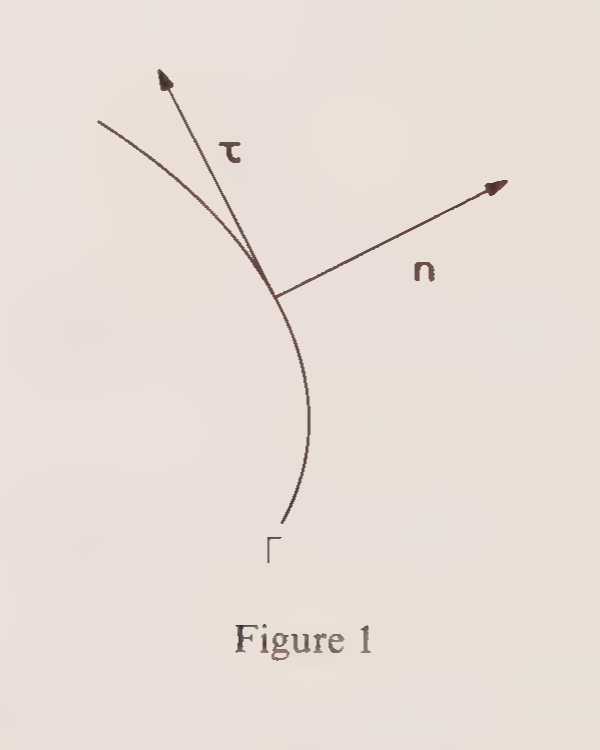
\includegraphics[width=.38\linewidth]{figures/figure-1.png}
\caption{二维边界上的外法向量与切向量.}\label{fig:sec2-normal-tangent}
\end{figure}

\setcounter{statement}{10}
\begin{Theorem}\label{thm:sec2-tangential-trace}
定义在 $\D(\overline\Omega)^N$ 上的映射
$\gamma_\tau:\mathbf v\mapsto\mathbf v\cdot\boldsymbol\tau|_\Gamma$(当 $N=2$) 或
$\gamma_\tau:\mathbf v\mapsto\mathbf v\times\mathbf n|_\Gamma$(当 $N=3$),
可连续延拓为线性连续映射, 延拓后仍记为 $\gamma_\tau$, 它将
$H(\Curl;\Omega)$ 映入 $H^{-1/2}(\Gamma)$(当 $N=2$) 或
$H^{-1/2}(\Gamma)^3$(当 $N=3$). 此外, 有 Green 公式
\begin{equation}\label{eq:sec2-hcurl-green}
\begin{aligned}
  (\Curl\mathbf v,\boldsymbol\phi)-(\mathbf v,\Curl\boldsymbol\phi)
  &=\langle\gamma_\tau\mathbf v,\boldsymbol\phi\rangle_\Gamma
  \quad\forall\mathbf v\in H(\Curl;\Omega),\\
  &\forall\boldsymbol\phi\in H^1(\Omega)^3\quad\text{if }N=3,\\
  &\text{or }\forall\phi\in H^1(\Omega)\quad\text{if }N=2.
\end{aligned}
\end{equation}
\end{Theorem}
证明与 Theorem~\ref{thm:sec2-normal-trace} 完全相似, 故略去. 为避免记号过多,
当 $N=2$ 或 $N=3$ 时, 分别把 $\gamma_\tau\mathbf v$ 记为
$\mathbf v\cdot\boldsymbol\tau|_\Gamma$ 或 $\mathbf v\times\mathbf n|_\Gamma$.
下面转向 $H(\Curl;\Omega)$ 中的 $\Ker(\gamma_\tau)$.

\SampleSourcePage{49}{35}
\setcounter{statement}{11}
\begin{Theorem}\label{thm:sec2-h0curl-kernel}
有
\[
  \Ker(\gamma_\tau)=H_0(\Curl;\Omega).
\]
\end{Theorem}
\begin{Proof}
在 \eqref{eq:sec2-hcurl-green} 中取极限, 显然有
$H_0(\Curl;\Omega)\subset\Ker(\gamma_\tau)$. 反向包含是
Lemma~\ref{lem:sec2-h0curl-characterization-test} 的直接应用.
\end{Proof}

\setcounter{statement}{2}
\begin{Remark}\label{rem:sec2-tangential-components}
向量场 $\mathbf v$ 在 $\Gamma$ 上的切向分量形式上定义为
\[
  \mathbf v_T=\mathbf v-(\mathbf v\cdot\mathbf n)\mathbf n.
\]
显然 $\mathbf v_T\times\mathbf n=\mathbf v\times\mathbf n$. 因而
$H(\Curl;\Omega)$ 中每个向量场 $\mathbf v$ 满足
$\mathbf v\times\mathbf n|_\Gamma=0$, 当且仅当它在 $\Gamma$ 上的切向分量为零.
类似地, $H^1(\Omega)$ 中每个函数 $q$ 满足
$(\Grad q)\times\mathbf n=0$ on $\Gamma$, 当且仅当 $q$ 在 $\Gamma$ 的每个连通分支上为常数.
\end{Remark}

\setcounter{statement}{3}
\begin{Remark}\label{rem:sec2-hcurl-hdiv-2d}
当 $N=2$ 时, $\mathbf v=(v_1,v_2)$ 属于 $H(\Curl;\Omega)$, 当且仅当
$\mathbf w=(-v_2,v_1)$ 属于 $H(\Div;\Omega)$. 此外,
$\mathbf w\cdot\mathbf n=-\mathbf v\cdot\boldsymbol\tau$. 因而
Theorems~\ref{thm:sec2-dense-in-hdiv}, \ref{thm:sec2-normal-trace},
\ref{thm:sec2-h0div-kernel} 和 Corollary~\ref{cor:sec2-normal-trace-surjective}
中关于 $H(\Div;\Omega)$ 的性质都直接转化为 $H(\Curl;\Omega)$ 的性质.
\end{Remark}

\setcounter{statement}{4}
\begin{Remark}\label{rem:sec2-curl-in-h}
若 $\mathbf v\in H_0(\Curl;\Omega)$, 则 $\Curl\mathbf v\in H$. 事实上,
由于 $\Div\Curl\mathbf v=0$, 只需验证
$(\Curl\mathbf v)\cdot\mathbf n=0$. 对 $\phi\in H^2(\Omega)$,
Green 公式 \eqref{eq:sec2-hdiv-green} 和 \eqref{eq:sec2-hcurl-green} 给出
\[
  \langle(\Curl\mathbf v)\cdot\mathbf n,\phi\rangle_\Gamma
  =\int_\Omega\Curl\mathbf v\cdot\Grad\phi\dd x
  =\langle\mathbf v\times\mathbf n,\Grad\phi\rangle_\Gamma=0.
\]
结论由 $H^2(\Omega)$ 在 $H^1(\Omega)$ 中的稠密性得到.
\end{Remark}

最后考察 $H_0(\Div;\Omega)$ 与 $H_0(\Curl;\Omega)$ 的交.

\setcounter{statement}{4}
\begin{Lemma}\label{lem:sec2-h1-hdiv-hcurl}
以下等式在代数和拓扑意义下成立:
\[
  H_0^1(\Omega)^N=H_0(\Div;\Omega)\cap H_0(\Curl;\Omega).
\]
\end{Lemma}
\begin{Proof}
对 $N=3$ 证明; $N=2$ 时证明类似且更简单. 令
$\mathbf v\in H_0(\Div;\Omega)\cap H_0(\Curl;\Omega)$, 并令
$\widetilde{\mathbf v}$ 是 $\mathbf v$ 在 $\Omega$ 外的零延拓. 由 Green 公式
\eqref{eq:sec2-hdiv-green} 和 \eqref{eq:sec2-hcurl-green}, 容易得到
$\widetilde{\mathbf v}\in H(\Div;\R^3)\cap H(\Curl;\R^3)$, 且
\[
\begin{gathered}
  \|\Div\widetilde{\mathbf v}\|_{0,\R^3}=\|\Div\mathbf v\|_{0,\Omega},\\
  \|\Curl\widetilde{\mathbf v}\|_{0,\R^3}=\|\Curl\mathbf v\|_{0,\Omega},\\
  \|\widetilde{\mathbf v}\|_{0,\R^3}=\|\mathbf v\|_{0,\Omega}.
\end{gathered}
\]

\SampleSourcePage{50}{36}
令 $\mathcal F\widetilde{\mathbf v}$ 表示 $\widetilde{\mathbf v}$ 的 Fourier 变换, 按通常方式定义为
\begin{equation}\label{eq:sec2-fourier-transform-vector}
  \mathcal F\widetilde{\mathbf v}(\boldsymbol\mu)
  =\int_{\R^3}e^{-2i\pi(x,\boldsymbol\mu)}
  \widetilde{\mathbf v}(x)\dd x,
\end{equation}
其中
\[
  (x,\boldsymbol\mu)=\sum_{i=1}^{3}x_i\mu_i.
\]
由 Fourier 变换的性质, 众所周知
$\mathcal F\widetilde{\mathbf v}\in L^2(\R^3)^3$, 且
\[
\begin{aligned}
  \|\mathcal F\widetilde{\mathbf v}\|_{0,\R^3}
    &=\|\mathbf v\|_{0,\Omega},\\
  \mathcal F(\Curl\widetilde{\mathbf v})
    &=2i\pi(\mu_2\mathcal F\widetilde v_3-\mu_3\mathcal F\widetilde v_2,
      \mu_3\mathcal F\widetilde v_1-\mu_1\mathcal F\widetilde v_3,
      \mu_1\mathcal F\widetilde v_2-\mu_2\mathcal F\widetilde v_1),\\
  \mathcal F(\Div\widetilde{\mathbf v})
    &=2i\pi(\mu_1\mathcal F\widetilde v_1+
      \mu_2\mathcal F\widetilde v_2+mu_3\mathcal F\widetilde v_3).
\end{aligned}
\]
由这两个关系立即得到
\[
  \|\mathcal F(\partial\widetilde v_i/\partial x_j)\|_{0,\R^3}^2
  \le\|\Div\mathbf v\|_{0,\Omega}^2+
  \|\Curl\mathbf v\|_{0,\Omega}^2.
\]
因此 $\widetilde{\mathbf v}\in H^1(\R^3)^3$, 从而
$\mathbf v\in H_0^1(\Omega)^3$. 此外
\[
  \|\mathbf v\|_{1,\Omega}=\|\widetilde{\mathbf v}\|_{1,\R^3}
  \le C(\|\mathbf v\|_{0,\Omega}^2+
  \|\Div\mathbf v\|_{0,\Omega}^2+
  \|\Curl\mathbf v\|_{0,\Omega}^2)^{1/2},
\]
其中 $C$ 与 $\Omega$ 无关. 反向包含及反向不等式显然成立.
\end{Proof}

下一个推论是 Lemma~\ref{lem:sec2-h1-hdiv-hcurl} 的简单结果.

\setcounter{statement}{9}
\begin{Corollary}\label{cor:sec2-local-h1-hdiv-hcurl}
设 $\Omega$ 是 $\R^N$ 的任意开子集, 且
$\mathbf v\in H(\Div;\Omega)\cap H(\Curl;\Omega)$. 则
$\mathbf v\in H_{\loc}^1(\Omega)^3$.
\end{Corollary}

\setcounter{statement}{5}
\begin{Remark}\label{rem:sec2-global-h1-hdiv-hcurl}
由 Lemma~\ref{lem:sec2-h1-hdiv-hcurl} 的证明可知, 在代数和拓扑意义下
\[
  H^1(\R^N)^N=H(\Div;\R^N)\cap H(\Curl;\R^N).
\]
\end{Remark}

\setcounter{statement}{6}
\begin{Remark}\label{rem:sec2-hdiv-hcurl-estimate}
Lemma~\ref{lem:sec2-h1-hdiv-hcurl} 与
Theorem~\ref{thm:peetre-tartar-compact-operator} 立即给出
\[
  \|\mathbf v\|_{1,\Omega}
  \le C(\|\Div\mathbf v\|_{0,\Omega}^2+
  \|\Curl\mathbf v\|_{0,\Omega}^2)^{1/2}
  \quad\forall\mathbf v\in H_0(\Div;\Omega)\cap H_0(\Curl;\Omega).
\]
\end{Remark}
